\documentclass[aspectratio=43]{beamer}
%% \documentclass[aspectratio=169]{beamer}
\usetheme[
  block=fill,
  background=light,
  titleformat=smallcaps,
  progressbar=frametitle,
  numbering=none,
]{metropolis}
\setbeamersize{text margin left=.7cm,text margin right=.7cm}
\usepackage{appendixnumberbeamer}

%%%%%%%%%%%%%%%%%%%%%%%%%%%%%%%%%%%%%%%%%%
%% Packages
%%%%%%%%%%%%%%%%%%%%%%%%%%%%%%%%%%%%%%%%%%

% Tikz
\usepackage{tikz}
\usetikzlibrary{arrows,positioning,matrix,fit,decorations.text}

% Colors
\usepackage{xcolor}

% Images
\usepackage{graphics}
\graphicspath{{img/}}
\usepackage{caption}

% Math
\usepackage{proof}

%%%%%%%%%%%%%%%%%%%%%%%%%%%%%%%%%%%%%%%%%%
%% Macros
%%%%%%%%%%%%%%%%%%%%%%%%%%%%%%%%%%%%%%%%%%
\renewcommand\alert[1]{\textcolor{mLightBrown}{#1}}
\newcommand\todo[1]{\textcolor{red}{#1}}

%% Counters for `enumerate`
\newcounter{saveenumi}
\newcommand{\seti}{\setcounter{saveenumi}{\value{enumi}}}
\newcommand{\conti}{\setcounter{enumi}{\value{saveenumi}}}


\renewcommand{\i}{\textit}  % Just to speed up typing: replace these in the final version
\renewcommand{\t}{\texttt}  % Just to speed up typing: replace these in the final version
\newcommand{\s}{\textsf}  % Just to speed up typing: replace these in the final version
\newcommand{\msf}[1]{\ensuremath{\mathsf{#1}}}
\newcommand{\mi}[1]{\ensuremath{\mathit{#1}}}


%% Various text macros
\newcommand{\true}{\textsf{true}}
\newcommand{\false}{\textsf{false}}

\newcommand{\hash}[1]{\ensuremath{#1^{\#}}}

\newcommand{\List}[1]{\ensuremath{\s{List}[#1]}}
\newcommand{\Set}[1]{\ensuremath{\s{Set}[#1]}}
\newcommand{\Map}[2]{\ensuremath{\s{Map}[#1,#2]}}
\newcommand{\Interval}[1]{\ensuremath{\s{Interval}[#1]}}
\newcommand{\extended}[1]{#1^\updownarrow}

\newcommand{\script}{\ensuremath{\s{Script}}}
\newcommand{\scriptAddr}{\msf{scriptAddr}}
\newcommand{\ptx}{\ensuremath{\s{TxInfo}}}
\newcommand{\toPtx}{\msf{toTxInfo}}

\newcommand{\toData}{\msf{toData}}
\newcommand{\fromData}{\msf{fromData}}

% Macros for eutxo things.
\newcommand{\TxId}{\ensuremath{\s{TxId}}}
\newcommand{\txId}{\msf{txId}}
\newcommand{\txrefid}{\mi{id}}
\newcommand{\Address}{\ensuremath{\s{Address}}}
\newcommand{\DataHash}{\ensuremath{\s{DataHash}}}
\newcommand{\idx}{\mi{index}}
\newcommand{\inputs}{\mi{inputs}}
\newcommand{\outputs}{\mi{outputs}}
\newcommand{\forge}{\mi{forge}}
\newcommand{\fee}{\mi{fee}}
\newcommand{\addr}{\mi{addr}}
\newcommand{\val}{\mi{value}}  %% \value is already defined

\newcommand{\validator}{\mi{validator}}
\newcommand{\redeemerVal}{\mi{redeemer}}
\newcommand{\dataVal}{\mi{data}}
\newcommand{\dataHsh}{\mi{dataHash}}
\newcommand{\dataWits}{\mi{dataWitnesses}}
\newcommand{\hashData}{\msf{dataHash}}
\newcommand{\validityInterval}{\mi{validityInterval}}
\newcommand{\Data}{\ensuremath{\s{Data}}}

\newcommand{\outputref}{\mi{outputRef}}
\newcommand{\txin}{\mi{in}}
\newcommand{\id}{\mi{id}}
\newcommand{\lookupTx}{\msf{lookupTx}}
\newcommand{\currentTick}{\msf{currentTick}}
\newcommand{\getSpent}{\msf{getSpentOutput}}

\newcommand{\tick}{\ensuremath{\s{Tick}}}
\newcommand{\spent}{\msf{spentOutputs}}
\newcommand{\unspent}{\msf{unspentOutputs}}
\newcommand{\txunspent}{\msf{unspentTxOutputs}}
\newcommand{\eutxotx}{\msf{Tx}}

\newcommand{\qty}{\ensuremath{\s{Quantity}}}
\newcommand{\token}{\ensuremath{\s{Token}}}
\newcommand{\currency}{\ensuremath{\s{CurrencyId}}}
\newcommand{\nativeCur}{\ensuremath{\mathrm{nativeC}}}
\newcommand{\nativeTok}{\ensuremath{\mathrm{nativeT}}}
\newcommand{\injectNative}{\ensuremath{\mathrm{inject}}}

\newcommand{\qtymap}{\ensuremath{\s{Quantities}}}

%% \newcommand\B{\ensuremath{\mathbb{B}}}
\newcommand\N{\ensuremath{\mathbb{N}}}
%% \newcommand\Z{\ensuremath{\mathbb{Z}}}
%% \renewcommand\H{\ensuremath{\mathbb{H}}}
%% \H is usually the Hungarian double acute accent
\newcommand{\emptyBs}{\ensuremath{\emptyset}}

\newcommand{\emptymap}{\ensuremath{\{\}}}

% multisig
\newcommand{\msc}{\mathrm{msc}}
\newcommand{\sig}{\mathit{sig}}
\newcommand{\sigs}{\mathit{sigs}}
\newcommand{\auth}{\mathrm{auth}}
\newcommand{\Holding}{\msf{Holding}}
\newcommand{\Collecting}[2]{\msf{Collecting}(#1, #2)}
\newcommand{\Propose}[1]{\msf{Propose}(#1)}
\newcommand{\Add}[1]{\msf{Add}(#1)}
\newcommand{\Cancel}{\msf{Cancel}}
\newcommand{\Pay}{\msf{Pay}}

% Names, for consistency
\newcommand{\UTXO}{UTXO}
\newcommand{\EUTXO}{E\UTXO{}}
\newcommand{\ExUTXO}{Extended \UTXO{}}
\newcommand{\CEM}{CEM}

% ------

\newcommand\isFinal{\msf{isFinal}}
\newcommand\step{\msf{step}}
\newcommand\satisfies{\msf{satisfies}}
\newcommand\checkOutputs{\msf{checkOutputs}}

\newcommand\mkValidator[1]{\msf{validator}_#1}
\newcommand\Sim[2]{\ensuremath{
#1 \sim #2
}}
\newcommand\CStep[3]{\ensuremath{
#1 \xrightarrow{\hspace{5pt} #2 \hspace{5pt}} (#1' , #3)
}}
\newcommand\LStep[2]{\ensuremath{
#1 \xrightarrow{\hspace{5pt} #2 \hspace{5pt}} #1'
}}
\newcommand\txeq{tx^\equiv}

%%%%%%%%%%%%%%%%%%%%%%%%%%%%%%%%%%%%%%%%%%
%% Fonts
%%%%%%%%%%%%%%%%%%%%%%%%%%%%%%%%%%%%%%%%%%
\usepackage{relsize}
\usepackage[tt=false]{libertine}
\usepackage[libertine]{newtxmath}

%----------------------------------------------------------------------------

\title{The Extended UTXO Model}
%\subtitle{}
\author{
Manuel M.T. Chakravarty, James Chapman, Kenneth MacKenzie, \\
Orestis Melkonian, Michael Peyton Jones, Philip Wadler \\[5pt]
(presented by \textbf{Alexander Nemish}) \\[10pt]
}
\date{February 14, 2020}
\titlegraphic{
\vspace*{7cm}
\begin{center}
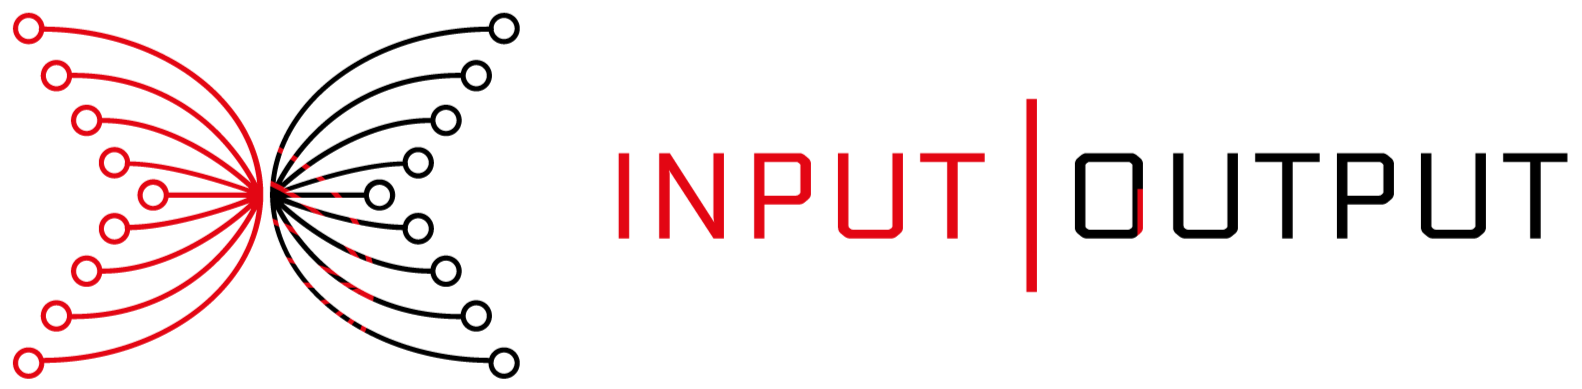
\includegraphics[keepaspectratio=true,height=1.4cm]{iohk}
\end{center}
}

\begin{document}
\begin{center}
\setbeamerfont{title}{size=\large}
\setbeamerfont{subtitle}{size=\small}
\maketitle
\setbeamerfont{title}{size=\Large}
\setbeamerfont{subtitle}{size=\large}
\end{center}

\tikzset{
  % global
  every matrix/.style =
  { ampersand replacement = \&,
    matrix of nodes,
    nodes in empty cells },
  % nodes
  boxx/.style = {align = center},
  box/.style =
  { %draw, rectangle,
    align          = center,
    minimum width  = .5cm,
    minimum height = 1.5cm },
  BG/.style =
  { rectangle,
    inner sep       = 0.2cm,
    rounded corners = 5mm,
    line width      = 1mm },
  MSc/.style =
  { BG, fill=yellow!25, text=yellow!25 },
  MSc-label/.style =
  { label={[name=msc]above left:\contour{yellow!25}{}} },
  PhD/.style =
  { BG, fill=orange!20, text=orange!20 },
  PhD-label/.style =
  { label={[name=phd]below:\contour{orange!20}{}} },
  PhD2/.style =
  { BG, fill=orange!30, text=orange!30 },
  PhD2-label/.style =
  { label={[name=phd]#1:\contour{orange!30}{}} },
  PhD3/.style =
  { BG, fill=green!25, text=green!25 },
  PhD3-label/.style =
  { label={[name=phd]#1:\contour{green!25}{}} },
  greenBox/.style =
  { BG, fill=green!15, },
%%   greenDot/.style =
%%   { BG , left color = red!35, middle color = green!55
%%   , bottom color = green!55, right color = green!55 },
  redDot/.style =
  { BG, draw=red!55, dashed },
  %% font=\small,
  txt/.style    = {align=center},
  note/.style   = {font=\small\itshape},
  accept/.style = {fill = green!15},
  reject/.style = {fill = red!15},
  cit/.style =
  { inner sep = 0.3cm, rounded corners = 2mm, font=\normalsize, align=center },
  % edges
  to/.style = {->, thick},
  squig/.style = {decorate, decoration={zigzag}}
}

\newcommand\bitml{
  \matrix (mat)
    [ column sep = 1.5cm,
      row sep = 2cm,
      every node/.style = txt
    ] {
    \node {\textbf{\underline{Syntax}}};
    \& \node (operA) {};
    \& \node (operB) {};
    \& \node {\textbf{\underline{Game-theoretic}}\\\textbf{\underline{Semantics}}}; \\[-1cm]
    \node (contracts) {BitML\\Contracts};
    \& \node (lts) {Small-step\\LTS};
    \& \node (sm) {Symbolic\\Runs};
    \& \node (ss) {Symbolic\\Strategies}; \\
    \node (transactions) {Bitcoin\\Transactions};
    \& \node (bc) {Blockchain\\Consistency};
    \& \node (cm) {Computational\\Runs};
    \& \node (cs) {Computational\\Strategies}; \\
  };
  \node[fit=(operA)(operB)]{\textbf{\underline{Operational Semantics}}};
  \path
  (contracts) edge[to]
    node[right] (comp) {$\mathcal{C}$}
  (transactions)
  (sm) edge[<->, bend left = 40]
    node[right] (coh) {$\sim$}
  (cm)
  (cm) edge[to]
    node[left] (parsing) {\textit{\alert{parse}}}
  (sm)
  (ss) edge[to]
    node[left] (n) {$\aleph$}
  (cs)
  (coh.east) edge[<->, double]
    node[above] (compsA) {\textit{\alert{computational}}}
    node[below] (compsB) {\textit{\alert{soundness}}}
  (n.west)
  (lts) edge[squig] (sm)
  (bc) edge[squig] (cm)
  ;
}

\newcommand\withLogo[2]{\raisebox{-.25\height}{\includegraphics[keepaspectratio=true,height=27pt]{#1}}~~#2}
\newcommand\no{\Large $\times$}
\newcommand\yes{\Large $\checkmark$}

\section{Introduction}
\begin{frame}[plain]


\renewcommand{\arraystretch}{2.5}
\begin{tabular}{l|l|c|c}
\textbf{\hfil\small Blockchain\hfil} & \textbf{\hfil\small Model\hfil} & \textbf{\small Turing-complete} & \textbf{\small Deterministic} \\
\hline
\withLogo{bitcoin}{Bitcoin} & UTXO & \no & \no \\
\hline
\hspace{3pt}\withLogo{ethereum}{\hspace{3pt}Ethereum} & Accounts & \yes & \no \\
\hline
\withLogo{ada}{Cardano (IOHK)} & EUTXO & \yes & \yes \\
\end{tabular}

\end{frame}

\begin{frame}{Methodology}
\begin{itemize}
\item Focus on validating the relevant meta-theory
  \begin{itemize}
  \item In contrast to validating individual contracts
  \end{itemize}
\item Fully mechanized approach, utilizing Agda's rich type system
\item Fits well with IOHK's research-oriented approach
\end{itemize}

\begin{tikzpicture}
  [basic box/.style = {
     draw,
     shape = rectangle,
     align = center,
     minimum width=2cm,
     minimum height=1.2cm,
     rounded corners},
   to/.style = {
     ->,
     >=stealth',
     semithick
  },
  every matrix/.style={column sep=.8cm, ampersand replacement=\&},
  font=\small
  ]
  \matrix{
     \node[basic box,draw=mLightBrown] (a) {pure\\ research};
  \& \node[basic box,draw=mLightBrown] (b) {mechanized\\ models};
  \& \node[basic box] (c) {reference\\ implementations};
  \& \node[basic box] (d) {production\\ code}; \\
  };

  \path
  (a) edge[to, mLightBrown] (b)
  (b) edge[to] (c)
  (c) edge[to] (d)
  ;
\end{tikzpicture}
\end{frame}

\begin{frame}[label=contributions]{Contributions}

\begin{itemize}
\setlength\itemsep{.25cm}

\item \textbf{Detailed description of the Extended UTXO model (EUTXO)}
\begin{center}
\scalebox{.7}{
  \begin{tikzpicture}
    \eutxo
  \end{tikzpicture}
}
\end{center}

\item \textbf{Formalization in} \raisebox{-.5\height}{
\includegraphics[height=.18\textheight]{agda}}\\

\item \textbf{Proof of bisimulation with a specific form of state machines}\\
\begin{center}
\scalebox{.6}{
  \begin{tikzpicture}
    \multisig
  \end{tikzpicture}
}
\end{center}

\end{itemize}

\end{frame}

\section{EUTXO, Informally...}

\begin{frame}{UTXO vs EUTXO}

\centering

\tikzset{
  tx/.style =
  { draw = gray,
    shape = rectangle,
    align = center,
    minimum width=.5cm,
    minimum height=1.5cm },
  mid/.style =
  { draw,
    yshift=.5cm,
    shape = circle,
    inner sep = 0pt,
    minimum size=4pt },
  math/.style =
  { yshift=-.5cm },
  arg/.style =
  { anchor=center,
    align=left,
    font=\scriptsize },
  to/.style =
  { -,
    bend left = 30,
    thick },
  every matrix/.style =
  { column sep=2.2cm,
    ampersand replacement=\& },
  font=\small
}

\begin{tikzpicture}
  \matrix (mat) [matrix of nodes, nodes in empty cells] {
     \node[mid,red]   (a) {};
  \& \node[tx]        (b) {};
  \& \node[mid,red]   (c) {};
  \& \node[tx]        (d) {};
  \& \node[mid,black] (e) {};
  \\ \& \& \& \& \\
  };
  \path
  (a) edge[to, red]
  (b)
  (b) edge[to, black] node[arg, yshift=-.7cm] {x : Value\\ $\nu$ : Validator}
  (c)
  (c) edge[to, red] node[arg, yshift=.4cm] {$\rho$ : Redeemer}
  (d)
  (d) edge[to, black]
  (e)
  ;
  \node[math,fit=(mat-2-1)(mat-2-5)]{$\nu(\rho) \overset{\text{\tiny ?}}{=} \s{True}$};
\end{tikzpicture}
\vspace{.5cm}
\noindent\hfil\rule{0.9\textwidth}{.4pt}\hfil
\begin{tikzpicture}
  \matrix (mat) [matrix of nodes, nodes in empty cells] {
     \node[mid,red]   (a) {};
  \& \node[tx]        (b) {};
  \& \node[mid,red]   (c) {};
  \& \node[tx,label=below:\scriptsize$\sigma$ : State] (d) {};
  \& \node[mid,black] (e) {};
  \\ \& \& \& \& \\
  };
  \path
  (a) edge[to, red]
  (b)
  (b) edge[to, black] node[arg, yshift=-1cm] {x : Value\\ $\nu$ : Validator\\ $\delta$ : Data}
  (c)
  (c) edge[to, red] node[arg, yshift=.4cm] {$\rho$ : Redeemer}
  (d)
  (d) edge[to, black]
  (e)
  ;
  \node[math,fit=(mat-2-1)(mat-2-5)]{$\nu(\rho,\ \delta,\ \sigma,\ x) \overset{\text{\tiny ?}}{=} \s{True}$};
\end{tikzpicture}

\end{frame}

\begin{frame}{Contract Continuity}
\begin{itemize}
\item New data value on outputs
\item More information available to validators
\item We show that Cardano can model a specific form of state machine
  \begin{itemize}
  \item However, much more computational patterns are possible
  \item e.g. the entirety of \alert{Marlowe}, a DSL for financial contracts, has
been implemented as a state machine on top of EUTXO.
  \end{itemize}
\end{itemize}
\end{frame}

\begin{frame}{Example: Multi-signature Contract}

\begin{itemize}
\item \textbf{n-out-of-m} signature scheme
\item Plain UTXO requires off-chain communication
\item Can be expressed as a simple state machine:
\end{itemize}

\centering
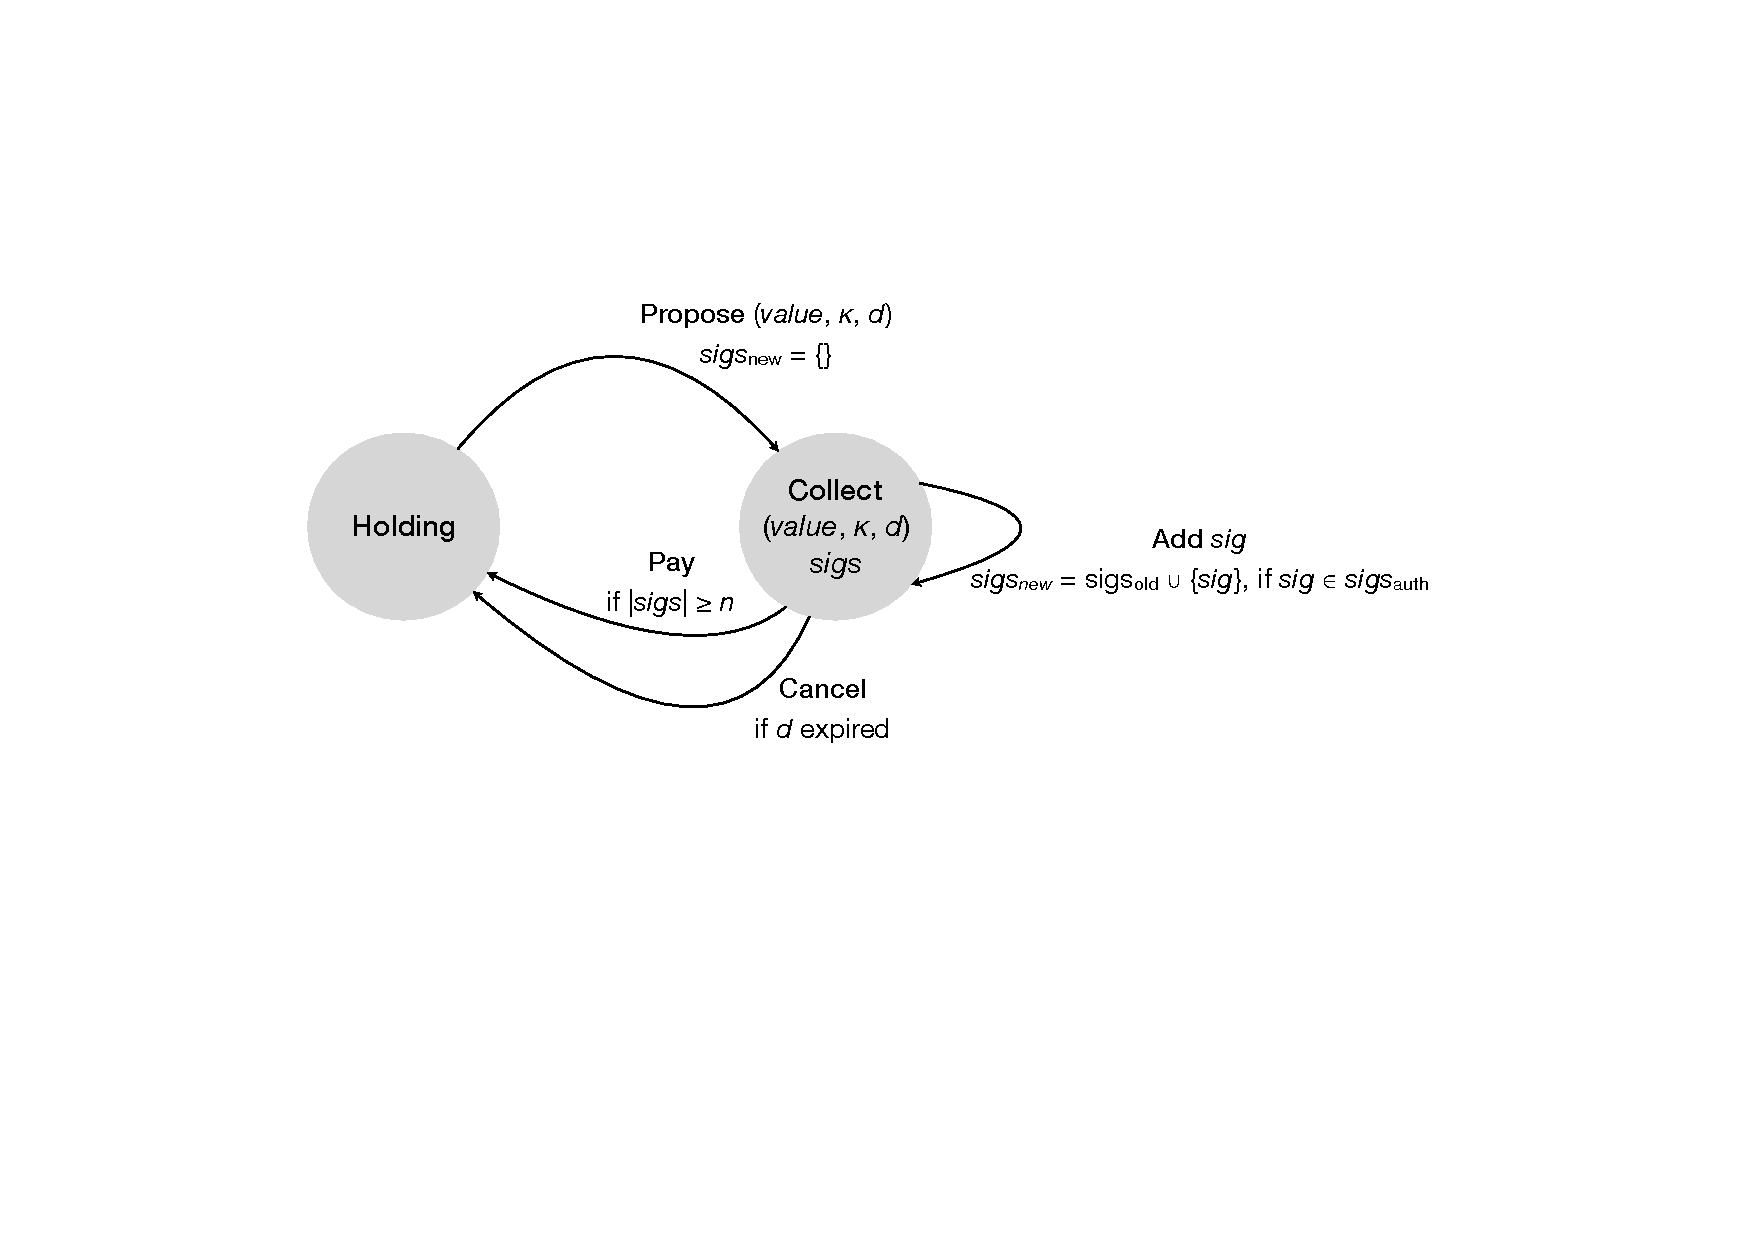
\includegraphics[width=\textwidth]{EUTxO_MultiSig_States.pdf}

\end{frame}

\begin{frame}{Example: Implementation in EUTXO}

\begin{itemize}
\item State machine is associated to a \textit{validator} function
\item \textit{Data values} in outputs correspond to states
  \begin{itemize}
  \item $\in \{ \msf{Holding} , \msf{Collecting} \}$
  \end{itemize}
\item Validator takes one of four possible transitions
  \begin{itemize}
  \item $\in \{ \msf{Propose} , \msf{Add} , \msf{Cancel} , \msf{Pay} \}$
  \item Choice provided by the \textit{redeemer} of the spending input
  \end{itemize}
\end{itemize}

\end{frame}

\section{EUTXO, Formally...}

\begin{frame}{Enhanced Scripting: Data Values \& Contract Continuity}

\begin{enumerate}
\item \alert{Data values} additionally carried by outputs
  \begin{itemize}
  \item passed as extra argument of type \s{Data} during validation
  \item allows a contract to carry data without changing its code
  \item otherwise we could not identify a contract by its code's hash
  \end{itemize}
\item More information about the transaction available to the validator
  \begin{itemize}
  \item passed as extra argument of type \s{TxInfo} during validation
  \item allows inspection of the transaction's outputs, thus supporting\\
\alert{contract continuity} (i.e. outputs use the expected validator)
  \end{itemize}
\seti
\end{enumerate}

\end{frame}

\begin{frame}{Enhanced Scripting: Validity Intervals \& Determinism}

\begin{enumerate}
\conti
\item Transactions have (restricted) access to time
  \begin{itemize}
  \item addition transaction field: \alert{validity interval}
  \item specifies a time interval, in which the transaction must be processed
  \item in contrast to allowing access to the current time
    \begin{itemize}
    \item allows for \alert{deterministic} script execution
    \item we can pre-calculate consumed resources/time
    \item a user can simulate execution locally
    \end{itemize}
  \end{itemize}
\end{enumerate}

\end{frame}

\begin{frame}{Validity of EUTXO Transactions (I)}

\begin{enumerate}
\item
  \label{rule:tick-in-range}
  \textbf{The current tick is within the validity interval}
  \begin{displaymath}
    \currentTick \in t.\validityInterval
  \end{displaymath}

\item
  \label{rule:all-outputs-are-non-negative}
  \textbf{All outputs have non-negative values}
  \begin{displaymath}
    \forall o \in t.\outputs,\ o.\val \geq 0
  \end{displaymath}

\item
  \label{rule:all-inputs-refer-to-unspent-outputs}
  \textbf{All inputs refer to unspent outputs}
  \begin{displaymath}
    \{i.\outputref : i \in t.\inputs \} \subseteq \unspent(l)
  \end{displaymath}

\item
  \label{rule:value-is-preserved}
  \textbf{Value is preserved (ignoring fees)}
  \begin{displaymath}
    \sum_{i \in t.\inputs} \getSpent(i, l).\val = \sum_{o \in t.\outputs} o.\val
  \end{displaymath}

\seti
\end{enumerate}

\end{frame}

\begin{frame}{Validity of EUTXO Transactions (II)}

\begin{enumerate}
\conti

\item
  \label{rule:no-double-spending}
  \textbf{No output is double spent}
  \begin{displaymath}
    \textrm{If } i_1, i_2 \in t.\inputs \textrm{ and }  i_1.\outputref = i_2.\outputref
    \textrm{ then } i_1 = i_2
  \end{displaymath}

\item
  \label{rule:all-inputs-validate}
  \textbf{All inputs validate}
  \begin{displaymath}
    \forall i \in t.\inputs,\ \llbracket
    i.\validator\rrbracket (i.\dataVal,\, i.\redeemerVal,\, \toPtx(t,i)) = \true
  \end{displaymath}

\item
  \label{rule:validator-scripts-hash}
  \textbf{Validator scripts match output addresses}
  \begin{displaymath}
    \forall i \in t.\inputs,\ \scriptAddr(i.\validator) = \getSpent(i, l).\addr
  \end{displaymath}

\item
  \label{rule:data-values-hash}
  \textbf{Data values match output hashes}
  \begin{displaymath}
    \forall i \in t.\inputs,\ \hashData(i.\dataVal) = \getSpent(i, l).\dataHsh
  \end{displaymath}
\end{enumerate}

\end{frame}

\section{Expressiveness of EUTXO}

\begin{frame}{Constraint Emitting Machines (CEM)}

To formally reason about the expressiveness of EUTXO, we introduce a specific form of state machines:
\begin{itemize}
\item Type of states \s{S}, type of inputs \s{I}
\item $\s{final} : \s{S} \rightarrow \s{Bool}$
\item $\s{step} : \s{S} \rightarrow \s{I} \rightarrow \s{Maybe}\ (\s{S} \times \s{TxConstraints})$
\end{itemize}

These are similar to Mealy machines, but differ in some aspects:
\begin{enumerate}
\item No notion of initial states
\item \textbf{Strictly} final states
\item Blockchain-specific output values (\s{TxConstraints})
\end{enumerate}

\end{frame}

\begin{frame}{Behavioural Equivalence: Notation}

\begin{itemize}
\item A ledger $l$ corresponds to a \CEM{} state $s$:
\[
\Sim{l}{s}
\]
\item New (valid) transaction submitted to ledger $l$:
\[
\LStep{l}{tx}
\]
\item Valid \CEM{} transition from source state $s$ to target state $s'$:
\[
\CStep{s}{i}{\txeq}
\]
\end{itemize}

\end{frame}

\begin{frame}{Transitions-as-transactions}

Given a smart contract, expressed as a \CEM{} $\mathcal{C}$,
we can derive the validator script that disallows any invalid transitions:
\[
\mkValidator{\mathcal{C}}(s, i, \mi{txInfo}) = \left\{
  \begin{array}{lll}
  \true  & \mi{if} \ \CStep{s}{i}{\txeq} \\
         & \mi{and} \ \satisfies(\mi{txInfo}, \txeq) \\
         & \mi{and} \ \checkOutputs(s', \mi{txInfo}) \\
  \false & \mi{otherwise}
  \end{array}
\right.
\]

\end{frame}

\begin{frame}{Behavioural Equivalence: Weak Bisimulation}

\begin{alertblock}{Proposition 1 (Soundness)}
Given a valid \CEM{} transition, we can construct a new valid transaction,
such that the resulting ledger corresponds to the target \CEM{} state:
\[
\infer[\textsc{sound}]
  {\exists tx\ l'\ .\ \LStep{l}{tx}\ \wedge \Sim{l'}{s'}}
  {%
    \CStep{s}{i}{\txeq}
  & \Sim{l}{s}
  }
\]
\end{alertblock}

\vfill

\begin{alertblock}{Proposition 2 (Completeness)}
Given a new valid transaction on the ledger, it is either irrelevant to the state machine
or corresponds to a valid \CEM{} transition:
\[
\infer[\textsc{complete}]
  { \Sim{l'}{s}\ \vee\ \exists i\ s'\ \txeq\ .\ \CStep{s}{i}{\txeq} }
  { \LStep{l}{tx}
  & \Sim{l}{s}
  }
\]
\end{alertblock}

\end{frame}

\begin{frame}{Related Work}

\begin{itemize}
\item \alert{Bitcoin Covenants}~~[Möser et al. @ FC'16]
  \begin{itemize}
  \item Allows restricting how output values will be used in the future
  \item Major inspiration for our introduction of \textit{data values}
  \end{itemize}
\item \alert{Bitcoin Modelling Language (BitML)}~~[Bartoletti et al. @ CCS'18]
  \begin{itemize}
  \item Process-calculus with automata-based operational semantics
  \item Compiles down to standard Bitcoin transactions
  \item Quite complicated translation and requires off-chain communication
  \end{itemize}
\item \alert{Scilla}~~[Sergey et al. @ OOPSLA'19]
  \begin{itemize}
  \item For Ethereum-like contracts, using \textit{communicating automata}
  \item Embedded in Coq, allows proving temporal (hyper-)properties
  \end{itemize}
\item \alert{Timed Automata}~~[Andrychowicz et al. @ FORMATS'14]
  \begin{itemize}
  \item Pragmatic model checking of Bitcoin contracts using \textsc{UPPAAL}
  \item Does not come with formal guarantees though
  \end{itemize}
\end{itemize}

\end{frame}

\againframe{contributions}


\begin{frame}[standout]
  Questions?
\end{frame}

\appendix
\newcommand\bs[1]{\mbox{\textbf{\s{#1}}}}

\begin{frame}{Ledger Primitives}

\begin{displaymath}
\begin{array}{rll}
  \bs{Quantity} && \mbox{an amount of currency}\\
  \bs{Tick}  && \mbox{a tick}\\
  \bs{Address} && \mbox{an ``address'' in the blockchain}\\
  \bs{Data}  && \mbox{a type of structured data}\\
  \bs{DataHash} && \mbox{the hash of a value of type \Data{}}\\
  \bs{TxId} && \mbox{the identifier of a transaction}\\
  \bs{txId} : \s{Tx} \rightarrow \s{TxId} && \mbox{get a transaction's identifier}\\
  \bs{Script} && \mbox{the (opaque) type of scripts}\\
  \bs{scriptAddr} : \s{Script} \rightarrow \s{Address} && \mbox{the address of a script (i.e. its hash)}\\
  \bs{dataHash} : \s{Data} \rightarrow \s{DataHash} && \mbox{the hash of a data value}\\
  \mathbf{\llbracket \_ \rrbracket} : \script \rightarrow \s{Args} \rightarrow \s{Bool} && \mbox{applying a script to its arguments}\\
\end{array}
\end{displaymath}

\end{frame}

\begin{frame}{Defined Types}

\begin{displaymath}
\begin{array}{rll}
  \bs{Output }    &=&(\val: \qty, \addr: \Address, \dataHsh: \DataHash)\\[8pt]

  \bs{OutputRef } &=&(\txrefid: \TxId, \idx: \N)\\[8pt]

  \bs{Input }     &=&(\outputref: \s{OutputRef}, \validator: \script,\\
                  & &\ \dataVal: \Data, \redeemerVal: \Data)\\[8pt]

  \bs{Tx }        &=&(\inputs: \Set{\s{Input}}, \outputs: \List{\s{Output}},\\
                  & &\ \validityInterval: \Interval{\tick})\\[8pt]

  \bs{Ledger }    &=&\!\List{\eutxotx}\\
\end{array}
\end{displaymath}

\end{frame}



\end{document}
